\section{Reconstrucción a partir de múltiples imágenes y odometría}

Al capturar un mismo entorno desde diversas imágenes distintas, tenemos un nuevo tipo de problema. Ahora, tenemos mucha más información espacial, que depende para cada imagen tanto de la región capturada como de la pose de la cámara.

\begin{figure}[H]
    \centering
    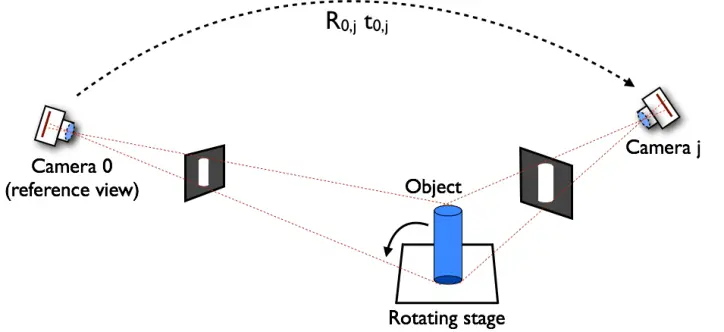
\includegraphics[width=1\linewidth]{../imagenes_marco_teorico/multiples_imagenes.png}
    \caption{Un mismo objeto capturado desde dos puntos. Las cámaras se diferencian por su pose. Imagen extraída de \cite{multiview_reconstruction_blog}.}
    \label{fig:multiview_reconstruction}
\end{figure}

Cada cámara tiene su propia rotación $\mathbf{R}$ y traslación $\mathbf{t}$, no están ordenadas y no tienen necesariamente los mismos parámetros intrínsecos. En la figura \ref{fig:multiview_reconstruction}, se observa este problema fijando una cámara como referencia y teniendo que encontrarse los parámetros de las demás respecto de la inicial. El abordaje de este problema se conoce como \textit{Structure from Motion} (SfM), tratado comúnmente de forma offline y con gran costo computacional. En la figura \ref{fig:rome16k} se observa un ejemplo de este tipo de reconstrucción a gran escala.

\begin{figure}[H]
    \centering
    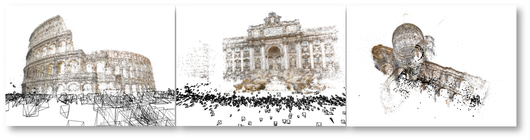
\includegraphics[width=1\linewidth]{../imagenes_marco_teorico/rome16k.png}
    \caption{Las más de dos millones de fotografías de edificios de Roma dieron lugar a un proyecto de reconstrucción llamado \textit{Building Rome in a Day}, llevando a gran escala la SfM. Imágenes extraídas de \cite{building_rome_agarwal}.}
    \label{fig:rome16k}
\end{figure}

Debido a la naturaleza de las imágenes a color, además, el mapa reconstruido no tiene ninguna noción de la escala real de los objetos. Esto se debe a que una imagen a color presenta una ambigüedad respecto a la distancia: por ejemplo de si se trata de un objeto cercano muy chico, o un objeto lejano muy grande \cite{sfm_scale_ambiguity}, como mencionamos anteriormente. Para tratar este problema, es necesario añadir información extra, por ejemplo fusionando la imagen a color con la información de otros sensores. En el marco de este trabajo, el mantenimiento de la escala real resulta crucial, y es gracias a las imágenes RGB-D que se elimina esta ambigüedad. Sin embargo, ambas cámaras están separadas en el espacio, por lo que resulta necesario un paso previo para fusionar las imágenes en una sola, alineando sus datos. Este proceso se conoce como registro.

Para ello, elegimos uno de los marcos relativos para expresar la imagen resultante. En este caso, el marco de la cámara a color, por lo que necesitamos registrar la profundidad. Luego, necesitamos datos previos sobre las intrínsecas de ambas cámaras, y las extrínsecas que llevan de una cámara a la otra. Con todo esto, una vez tomamos una imagen a color y una de profundidad, utilizamos la proyección inversa con las intrínsecas de la cámara de profundidad para llevar los puntos bidimensionales desde el plano de la cámara de profundidad hacia el espacio, expresado en el marco de esta misma cámara. Luego, con las extrínsecas pasamos hacia el marco de la cámara de color transformando todos los puntos, tras lo cual utilizamos los datos de las intrínsecas para pasar al plano de la cámara a color. Este procedimiento se observa en la figura \ref{fig:rgbd_registration}.

\begin{figure}[H]
    \centering
    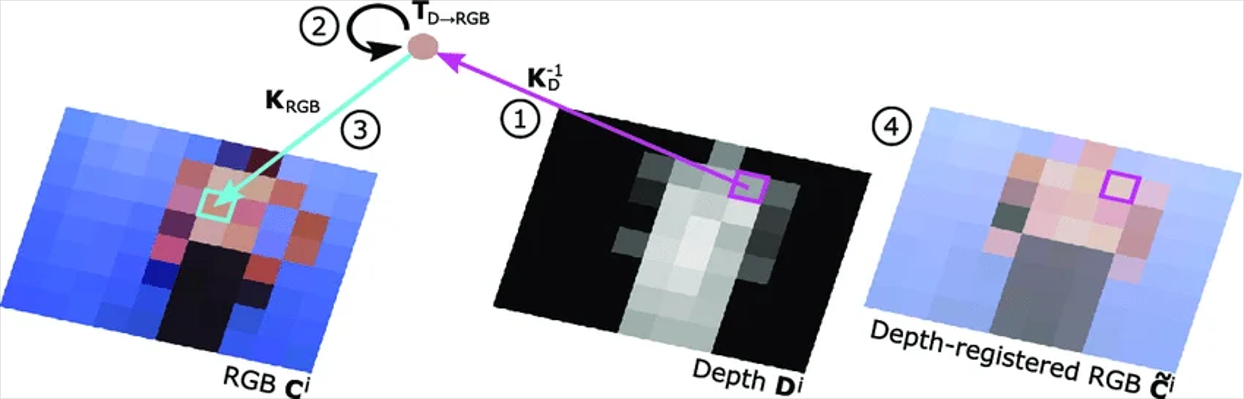
\includegraphics[width=0.75\linewidth]{../imagenes_marco_teorico/rgbd_registration.png}
    \caption{Registrado de un píxel particular, usando las intrínsecas $\mathbf{K}$ y extrínsecas $\mathbf{T}$. Imagen extraída de \cite{rgbd_registration}.}
    \label{fig:rgbd_registration}
\end{figure}

